\section{TRAJECTORY GENERATION}\label{method}
%
In table tennis, one needs to specify when, where and how to intercept the incoming ball trajectory $\ball(t)$. So far, most of the algorithms for robotic table tennis \cite{Matsushima05}, \cite{Muelling13} calculate the intersection point of an estimated ball trajectory $\ballEst(t)$ with a virtual hitting plane $y = y_{\mathrm{VHP}}$ to determine the space and time coordinates of the hitting point. It is possible to eliminate this plane altogether and include the striking time as another parameter to be determined in an optimization problem.
%
\subsection{Optimal Control for Trajectory Generation}
%
When generating striking trajectories for the robot, trajectories with minimal acceleration can be preferred for safety and efficiency reasons. We therefore consider the following \emph{free-time} optimal control problem~\cite{Liberzon11}
%
\begin{align}
&\min_{\ddot{\joint},T} \int\limits_{0}^{T}\ddot{\joint}(t)^{\mathrm{T}}\vec{R}\ddot{\joint}(t) \ \mathrm{d}t, \label{costFnc1} \\
\textrm{s.t. \ } & \kin_p(\joint(T)) = \ballEst(T), \label{transCond1} \\
& \kin_n(\joint(T)) = \normal_{\mathrm{des}}(T), \label{transCond2}\\
&\jac(\joint(T))\dot{\joint}(T) = \racketVel_{\mathrm{des}}(T), \label{transCond3} \\
&\joint(0) = \joint_{0}, \label{initCond1} \\
&\dot{\joint}(0) = \dot{\joint}_{0}, \label{initCond2}
\end{align}
%
\noindent where the final time $T$ of the racket trajectory is an additional variable to be optimized along with the joint accelerations $\ddot{\joint}(t) \in \mathbb{R}^{n}$. The vector-valued functions $\kin_p(\cdot), \kin_b(\cdot) \in \mathbb{R}^{3 \times 1}$ are the relevant submatrices of the direct kinematics function~\cite{Spong06} giving the racket normal $\normal(T)$ and racket center position $\racket(T)$ at striking time $T$ respectively. The Jacobian $\jac(\joint(T)) \in \mathbb{R}^{3 \times n}$ for the linear velocities gives the condition for the desired racket velocities $\racketVel_{\mathrm{des}}$. $\vec{R} \succ 0 \in \mathbb{R}^{n \times n}$ is a positive definite weighting matrix for the accelerations. Initial conditions for the robot are the joint positions $\joint_0$ and joint velocities $\dot{\joint}_0$.
%$\vec{T}(\cdot) \in \mathbb{R}^{4 \times 4}$ 

Solutions of \eqref{costFnc1} can be found using Pontryagin's maximum principle~\cite{Pontryagin}. In the appendix we show that the optimal $\joint(t)$ is a third degree polynomial for each degree of freedom, with the equality constraints \eqref{transCond1} - \eqref{transCond3} imposing a \emph{transversality condition} on the Hamiltonian and the momenta to satisfy at striking time~\cite{Schaettler12}. %See Figure~\ref{mainIdea} for an illustration.

When given only boundary equality constraints, the striking time $T$, the joint position and velocity values at striking time $\joint_f$ and $\dot{\joint}_f$ fully parametrize this problem. The optimal trajectory $\joint_{\mathrm{strike}}(t)$ can then be determined by solving a $2n+1$ nonlinear equations simultaneously. Inspired by the simplicity of this solution we extend the same parametrization to inequality-constrained optimization. In addition to the equality-constraints we consider joint position, velocity and acceleration limits imposed throughout the whole trajectory.

After computing the optimal values for $T, \joint_f, \dot{\joint}_f$, we generate also a returning trajectory $\joint_{\mathrm{return}}(t)$ to the same initial posture $\joint_0$ with an appropriately chosen return time $T_{\mathrm{return}}$ to guarantee feasibility. Initially the robot is not moving, $\dot{\joint}_0 = 0$.

\subsection{Predicting with Probabilistic Modeling}\label{sectionPredict}
 
In this framework, we require three models to determine the equality constraints~\eqref{transCond1} - \eqref{transCond3} for the trajectory generation process. We first need to predict the ball trajectory $\ballEst(t)$ for the ball $\ball = (b_x,b_y,b_z)^{\mathrm{T}}$ in midair from noisy ball observations. Table tennis balls are very light, a standard ball weighs about $2.7$ grams, which makes nonlinear effects due to air drag noticeable especially when the ball speed $\ballVel = \|\dot{\ball}\|_2$ is high. We use the ballistic \emph{flight model} 
%
\begin{align}
\begin{bmatrix}
   \ddot{b_x} \\
   \ddot{b_y} \\
   \ddot{b_z}   
 \end{bmatrix} &= 
 \begin{bmatrix}
 -\drag \ballVel \dot{b}_x  \\
 -\drag \ballVel \dot{b}_y  \\
 \ \gravity - \drag \ballVel \dot{b}_z 
 \end{bmatrix},
\label{flightModel}
\end{align}
%
\noindent which is a nonlinear dynamics model that incorporates air drag $\drag$ as well as gravity~$\gravity$. %$\ddot{\ball} = \ballDynamics(\dot{\ball})$ 

Formally, rebound is a discrete event which reflects the ball when the ball is touching the table. The incoming velocities  $\dot{\ball}_{\mathrm{in}}$ at bouncing time are transformed to outgoing velocities $\dot{\ball}_{\mathrm{out}}$. We use the linear \emph{rebound model}
%
\begin{align}
\dot{\ball}_{\mathrm{out}} = \bounce\dot{\ball}_{\mathrm{in}}.
\label{reboundModel}
\end{align}
%
Matrix $\bounce$ in \eqref{reboundModel} is a diagonal matrix with entries $\vec{\epsilon} = [\epsilon_{x}, \epsilon_{y}, -\epsilon_{z}]^{\mathrm{T}}$. The coefficient of restitution $\epsilon_{z} \in (0,1)$ accounts for the reflection of velocity in the vertical direction $z$ and $\epsilon_{x}, \epsilon_{y} \in (0,1)$ are the coefficients of friction along the planar $x,y$ directions. See Figure~\ref{models} for a table tennis schema. 
% this schema is no longer super relevant

\begin{figure}[t!]
\centering
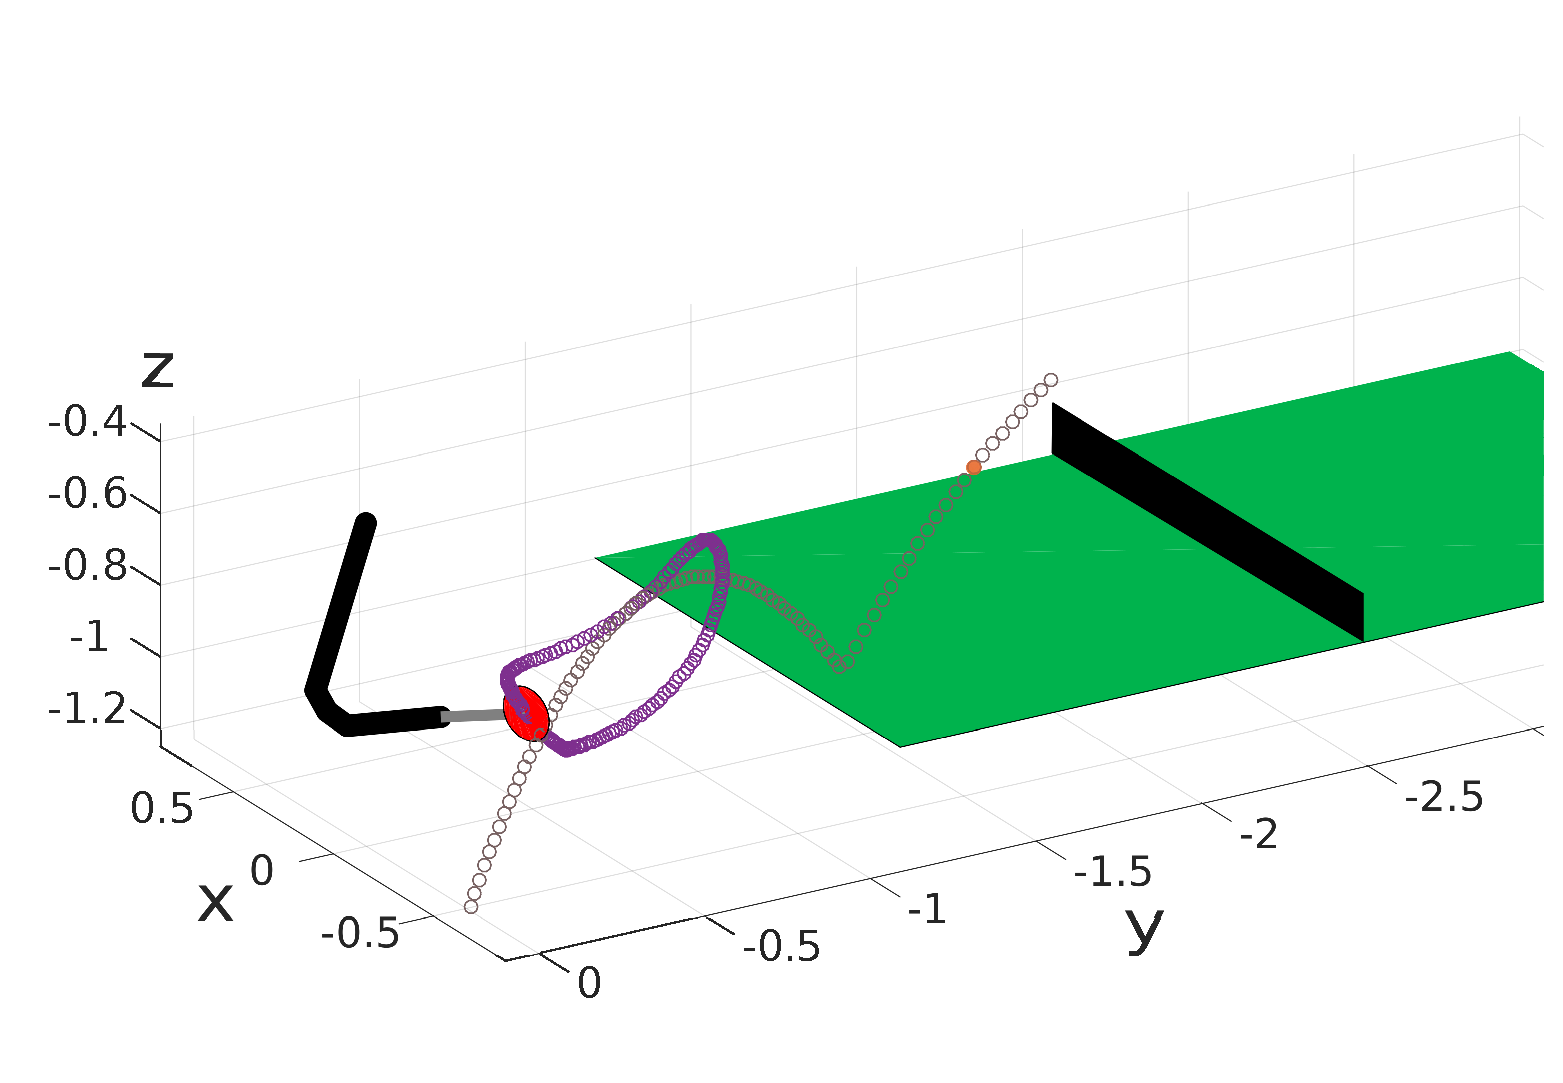
\includegraphics[scale=0.30]{tableTennis3D2.eps}			
\caption{A schema for a three dimensional table tennis model. Ball is shown as an orange blob and the racket, in resting state, is shown in red. We predict the path of the ball using the ballistic flight model, the rebound model and the racket-ball contact model respectively. The trajectory generation framework takes as input a desired racket trajectory calculated using these models. The predicted ball path and the generated robot trajectory are shown in gray and purple, respectively.}
\label{models}
\end{figure}

% should we move this to the algorithm section?
The accuracy of the rebound model~\eqref{reboundModel} clearly depends on that of the flight model~\eqref{flightModel}, so we first estimate the parameters of the flight model using nonlinear least squares on ball data before rebound. We then use the learned flight model to smoothen the ball path before rebound and after rebound. Using an Extended Kalman Smoother~\cite{Sorenson85}, we calculate the ball velocities before and after rebound and use linear least squares to estimate the rebound parameters. See Figure~\ref{trainBounce} for an illustration. Another approach would be to estimate the two model parameters together with a smoothing Expectation-Maximization (EM)~\cite{Shumway82} algorithm, yielding additionally covariance estimates for noisy ball observations. 

\begin{figure}[t!]
\centering
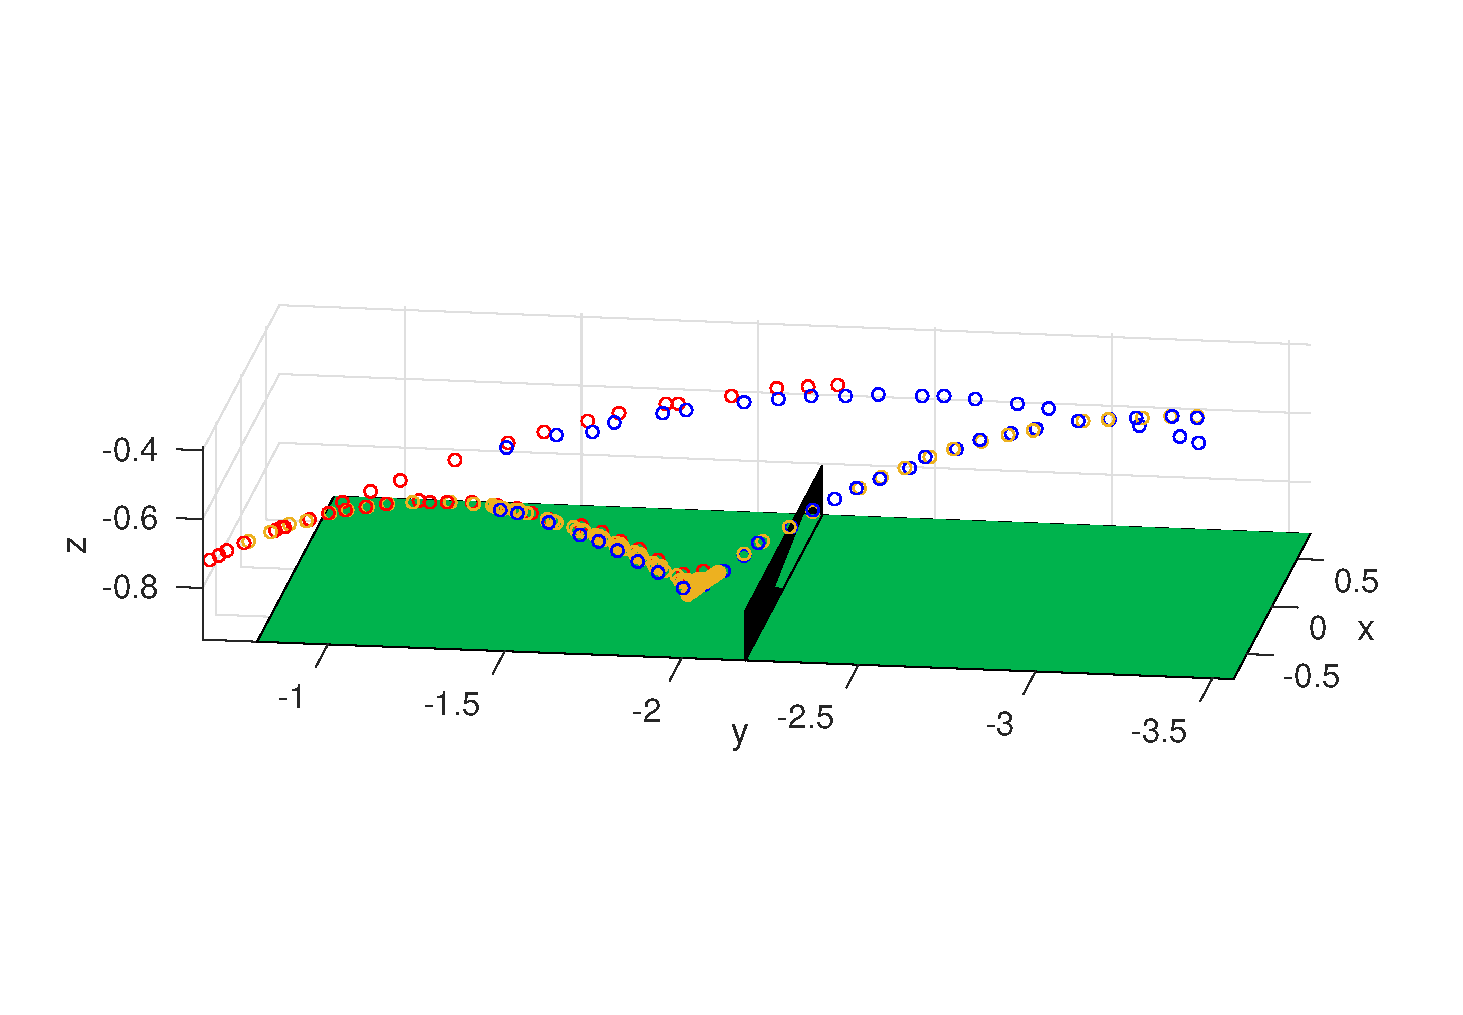
\includegraphics[scale=0.38]{trainBounce.eps}			
\caption{Using Extended Kalman Smoothing (EKS) to estimate the parameters of a linear rebound model from actual noisy ball data during a demonstration recording. Ball observations are acquired from two different sets of cameras on opposite sides of the table, shown as red and blue circles respectively. They are then smoothened with the EKS, shown in yellow, to obtain velocity estimates before rebound and just after rebound.} 
\label{trainBounce}
\end{figure}

\begin{figure}
  \begin{subfigure}[b]{0.16\textwidth}
    \centering
    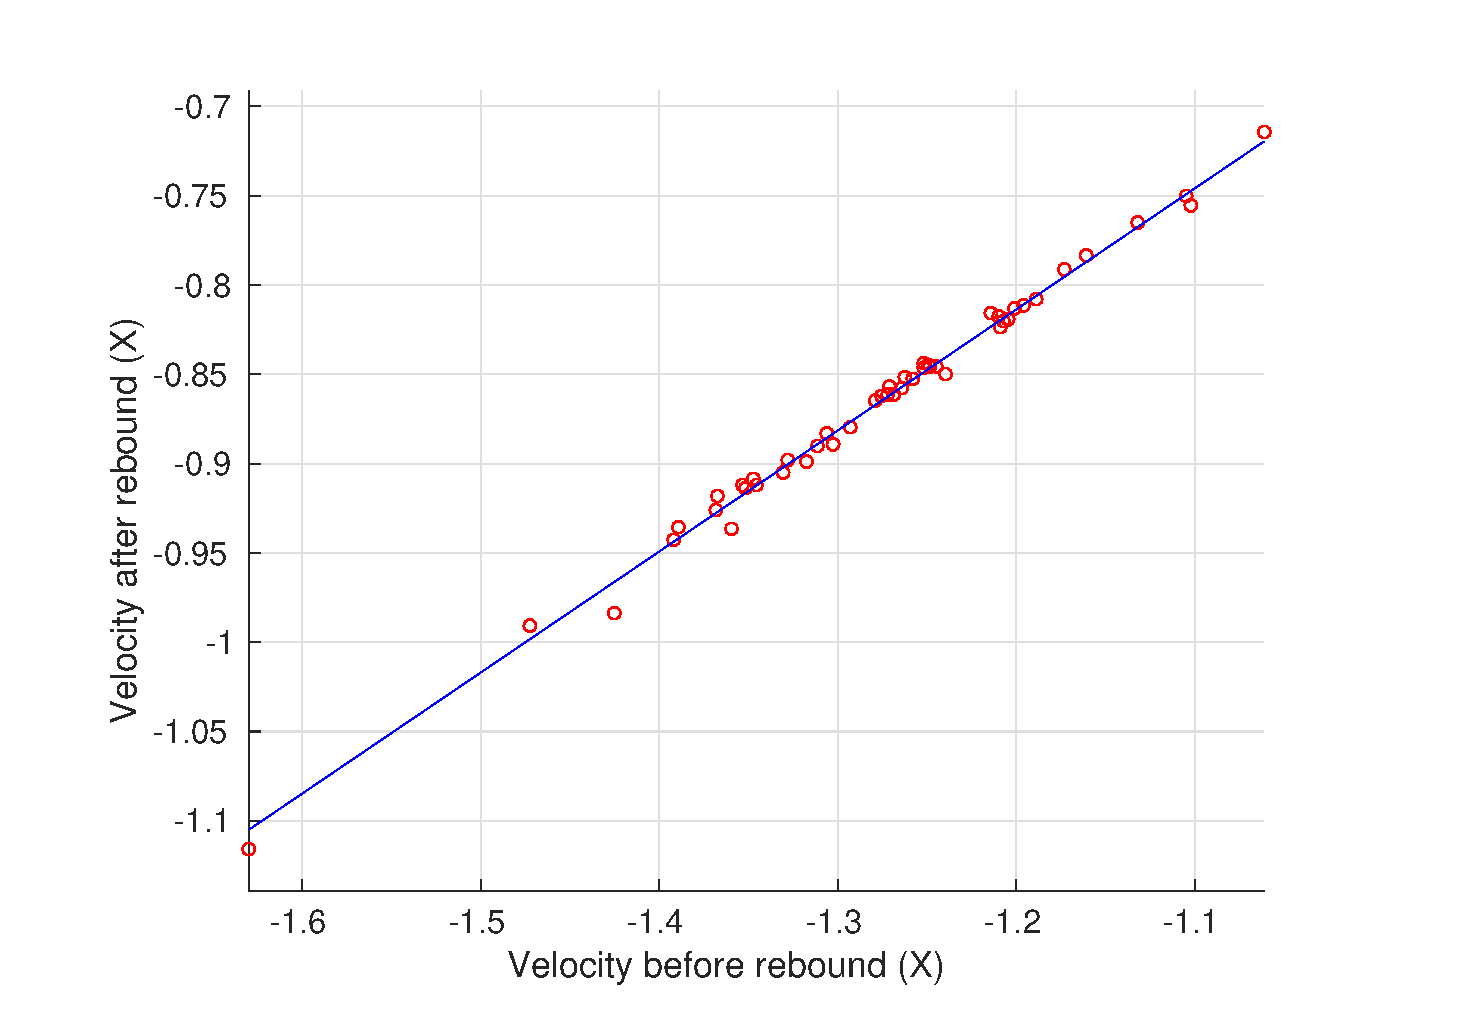
\includegraphics[width=\textwidth]{velXRebound.eps}
    \caption{X direction}
    \label{fig:1}
  \end{subfigure}\begin{subfigure}[b]{0.16\textwidth}
  	\centering
    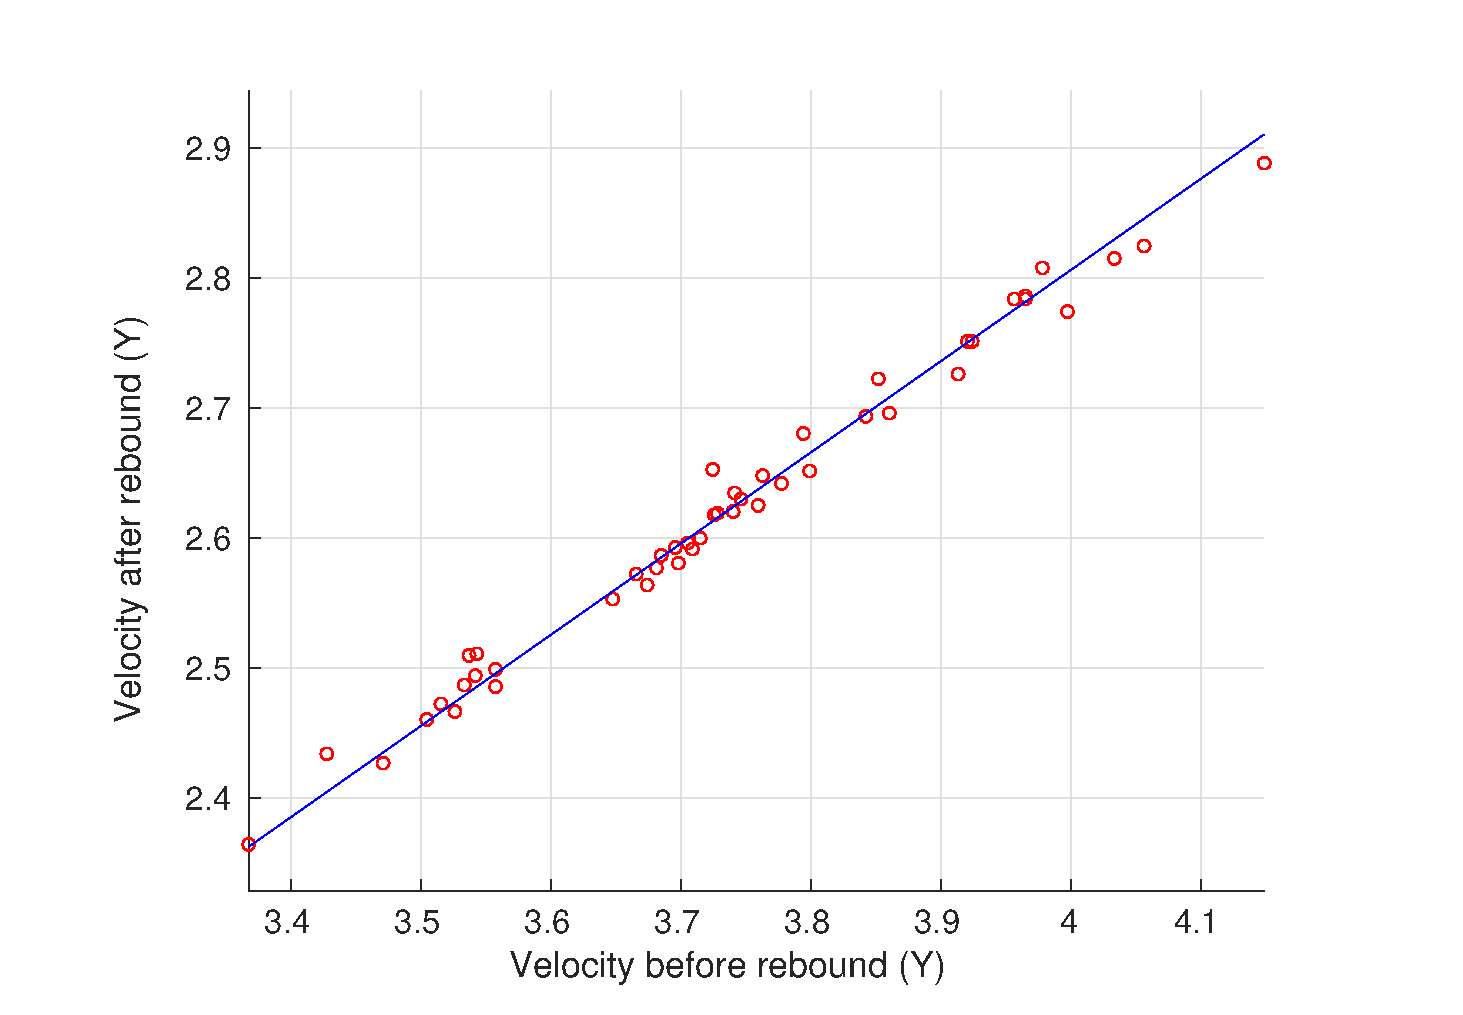
\includegraphics[width=\textwidth]{velYRebound.eps}
    \caption{Y direction}
    \label{fig:2}
  \end{subfigure}\begin{subfigure}[b]{0.16\textwidth}
    	\centering
      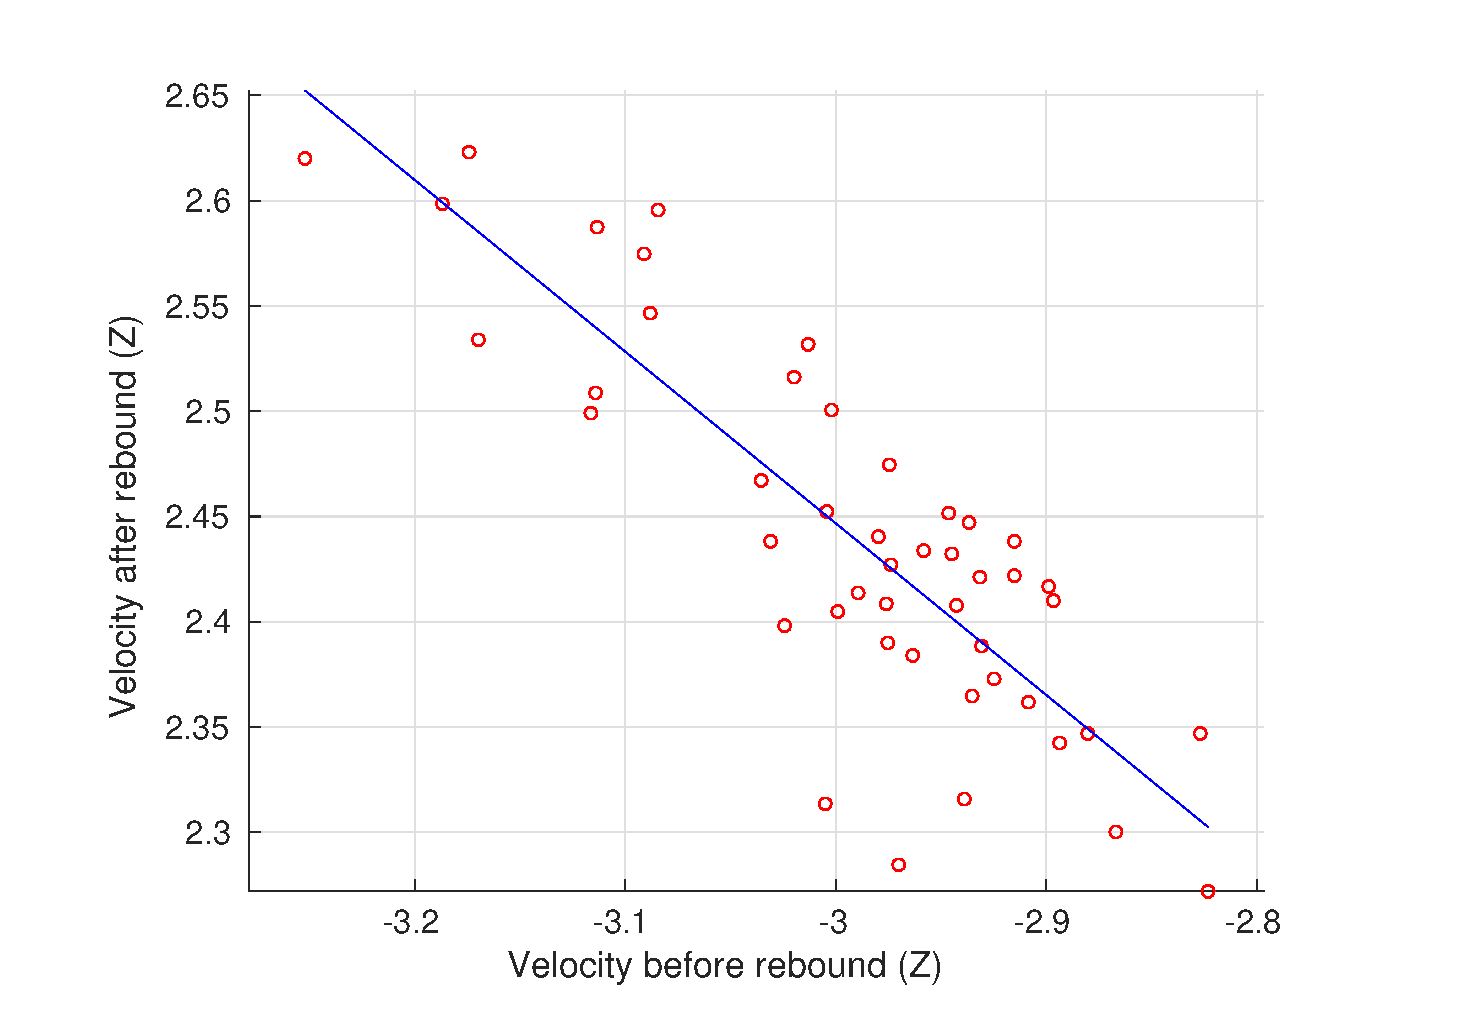
\includegraphics[width=\textwidth]{velZRebound.eps}
      \caption{Z direction}
      \label{fig:2}
    \end{subfigure}
  \caption{The plots show the relationship between the velocities before and after rebound. Estimating rebound model parameters from data with linear regression, we see that especially in the X and Y directions the linear model seems to be quite faithful to data. The topspin caused by our ball-launcher could be a complicating factor in the vertical direction Z. The estimated coefficients are $\epsilon_x = 0.8156$, $\epsilon_y = 0.7016$ and $\epsilon_z = 0.6780$.}
  \label{fig:rebound}
\end{figure}

%Effects of ball angular velocity, or in other words spin, are not accounted for in these models.

During test time we use Extended Kalman Filter (EKF)~\cite{Sorenson85} to perform prediction on the filtered ball state. 
% Any other regression method to estimate initial ball position and velocity can also be used. 
Using an EKF for our nonlinear model \eqref{flightModel} generates at each time instant $t$ a probability distribution $p_t(\ball,\dot{\ball}|t)$ of incoming ball states parameterized by time, 
%
\begin{align}
\ball(t) &\sim \mathcal{N}(\vec{\mu}_{\mathrm{est}},\vec{\Sigma}_{\mathrm{est}}(t)),
\label{ballProcess}
\end{align}
%
\noindent where $\vec{\mu}_{\mathrm{est}} = (\ballEst,\dot{\vec{b}}_{\mathrm{est}})$ is the mean ball position and velocity estimates.

In previous works~\cite{Muelling13}, the outgoing velocity of the ball as a result of contact is calculated using a \emph{mirror law}: 
%
\begin{align}
o_{n} - v_{n} = -\epsilon_{R} (i_{n} - v_{n}),
\label{mirrorLaw}
\end{align}
%
\noindent with $v_{n}$ the speed of the racket along its normal $\normal(t)$ and $\epsilon_{R} \in (0,1)$ the coefficient of restitution of the racket. Scalars $o_{n}$ and $i_{n}$ are the outgoing and incoming ball speeds along the racket normal, respectively. This model \eqref{mirrorLaw} assumes an elastic momentum exchange and it is quite inaccurate, especially at high ball velocities. Strategies to calculate $\normal_{\mathrm{des}}(t), \racketVel_{\mathrm{des}}(t)$ that use such simplistic modeling can render any trajectory generation framework claiming to be optimal, ineffective. Instead we estimate the parameters of a more general linear model
%
\begin{align}
\dot{\ball}_{\mathrm{out}} = \contactModel [\dot{\mathbf{b}}_{\mathrm{in}}^{\mathrm{T}},\dot{\racketVel}_{\mathrm{des}}^{\mathrm{T}}, \normal_{\mathrm{des}}^{\mathrm{T}}]^{\mathrm{T}}.
\label{contactModel}
\end{align}
%
Given a noisy dataset of human table tennis demonstrations $\dataset = \{\vec{t}_i, \ball_i, \joint_i\}_{i=1}^{N}$ of $N$ trials where each trial contains $M_i$ ball and $K_i$ joint values ordered by time, i.e. $\ball_i = \{\ball_{ij}\}_{j=1}^{j=M_i}, \joint_i = \{\joint_{ij}\}_{j=1}^{j=K_i}$, we can estimate the parameters of \eqref{contactModel} using linear regression. First we estimate the striking times by considering the minimum distance between the ball samples and the demonstrated robot trajectories
%
\begin{align}
j^{*} &= \arg\min_{j} \|\ball_{ij} - \kin_p(\joint_{ij})\|_2, \\
\hitTime &\approx \vec{t}_i(j^*),
\label{strikingTimeEst}
\end{align}
%
\noindent for each $i = 1, \ldots N$. Then as in estimating the rebound model, we use the Extended Kalman Smoother and smoothen the ball demonstrations before and after the striking time. This procedure results in estimating the incoming and outgoing ball velocities at striking time.

% put a figure here illustrating the idea

%The incoming ball mean $\ballEst(t)$ and covariance $\vec{\Sigma}_{\mathrm{est}}(t)$ of the normal distribution can be used to generate task-space strategies $\normal_{\mathrm{des}}(t), \racketVel_{\mathrm{des}}(t)$ to return the ball in a more cautious way. Given a noisy dataset of human table-tennis demonstrations of size $N$, i.e. $\dataset = \{\ball(\hitTime^i), \dot{\ball}(\hitTime^i), \racketVel(\hitTime^i), \normal(\hitTime^i), \ball(\landTime^i)\}_{i=1}^{N}$ we can train a probabilistic model between human-ball interactions $\dataMatrix = \{\ball(\hitTime^i), \dot{\ball}(\hitTime^i), \racketVel(\hitTime^i), \normal(\hitTime^i)\}_{i=1}^{N} \in \mathbb{R}^{N \times 12}$ and ball landing locations $\observations = \{b_x(\landTime^i), b_y(\landTime^i)\}_{i=1}^{N} \in \mathbb{R}^{N \times 2}$. The striking time $\hitTime$ and the landing time $\landTime$ denote the times when the racket intercepts the ball and the ball bounces on the table, respectively.  	

